\documentclass[output=paper,modfonts,nonflat]{langsci/langscibook} 
\ChapterDOI{10.5281/zenodo.1469573}

\title{Exploiting multilingual lexical resources to predict MWE compositionality} 

\author{Bahar Salehi\affiliation{The University of Melbourne}\and Paul Cook\affiliation{University of New Brunswick} \lastand Timothy Baldwin\affiliation{The University of Melbourne} }

\hyphenation{Swe-dish}

\abstract{Semantic idiomaticity is the extent to which the meaning of  a multiword expression (MWE) cannot be predicted from the meanings  of its component words. Much work in natural language processing on   semantic idiomaticity has focused on compositionality prediction,  wherein a binary or continuous-valued compositionality score is  predicted for an MWE as a whole, or its individual component   words. One source of information for making compositionality  predictions is the translation of an MWE into other languages.  This  chapter extends two previously-presented studies --   \cite{salehi2013} and \cite{DBLP:conf/eacl/SalehiCB14} -- that  propose methods for predicting compositionality that exploit  translation information provided by multilingual lexical resources,   and that are applicable to many kinds of MWEs in a wide range of  languages. These methods make use of distributional similarity of an  MWE and its component words under translation into many languages,   as well as string similarity measures applied to definitions of  translations of an MWE and its component words.  We evaluate these  methods over English noun compounds, English verb-particle   constructions, and German noun compounds. We show that the  estimation of compositionality is improved when using translations  into multiple languages, as compared to simply using distributional   similarity in the source language. We further find that string  similarity complements distributional similarity.  }
\begin{document}

\maketitle
\label{SALEHI-CHAPTER}



\section{Compositionality of MWEs\label{salehi:sec:intro}}


Multiword expressions (hereafter MWEs) are combinations of words which
are lexically, syntactically, semantically or statistically
idiosyncratic \citep{Sag2002a,baldwin2010multiword}. Much research has
been carried out on the extraction and identification of
MWEs\footnote{In this chapter, we follow \citet{baldwin2010multiword} in
  considering MWE ``identification'' to be a token-level
  disambiguation task, and MWE ``extraction'' to be a type-level
  lexicon induction task.} in \ili{English}
\citep{Schone2001,Pecina2008,fazly-cook-stevenson:2009:CL} and other languages
\citep{dias2003,evert2005,salehi2012}. However, considerably less work
has addressed the task of predicting the meaning of MWEs, especially
in non-\ili{English} languages. As a step in this direction, the focus of
this study is on predicting the compositionality\is{multiword expression!compositionality} of MWEs.

An MWE is fully compositional if its meaning is predictable from its
component words, and it is non-compositional\is{non-compositionality!semantic} (or idiomatic) if
not. For example, \localex{stand up} \gl{rise to one's feet} is
compositional, because its meaning is clear from the meaning of the
components \localex{stand} and \localex{up}. However, the meaning of
\localex{strike up} \gl{to start playing} is largely unpredictable
from the component words \localex{strike} and \localex{up}.

In this study, following \citet{mccarthy2003} and
\citet{reddy2011a}, we consider compositionality\is{multiword expression!compositionality} to be graded, and aim
to predict the \textit{degree} of compositionality\is{multiword expression!compositionality}. For example, in the
dataset of \citet{reddy2011a}, \localex{climate change} is judged to be
99\% compositional, while \localex{silver screen} is 48\% compositional and
\localex{ivory tower} is 9\% compositional. Formally, we model
compositionality\is{multiword expression!compositionality} prediction as a regression task.

An explicit handling of MWEs has been shown to be useful in NLP
applications \citep{ramisch2012}. As an example, \citet{carpuat2010}
proposed two strategies for integrating MWEs into statistical machine
translation. They show that even a large scale bilingual corpus cannot
capture all the necessary information to translate MWEs, and that in
adding the facility to model the compositionality\is{multiword expression!compositionality} of MWEs into their
system, they could improve translation quality. \citet{acosta2011}
showed that treating non-compositional MWEs as a single unit in
information retrieval improves retrieval effectiveness. For example,
while searching for documents related to \localex{ivory tower}, we are
almost certainly not interested in documents relating to elephant
tusks.

\largerpage
Our approach is to use a large-scale multi-way translation lexicon to
source translations of a given MWE and each of its component words,
and then model the semantic similarity between each component word and
the MWE.\footnote{Note that we will always assume that there are two
  component words, but the method is easily generalisable to MWEs with
  more than two components.} We consider similarity measures based on
\isi{distributional similarity} from monolingual corpora for the source
language and each of the target languages, as well as string
similarity measures applied to definitions of translations of an MWE
and its component words as shown in \figref{fig:diagram}. We then
consider a variety of approaches to combining similarity scores from
the various languages to produce a final compositionality\is{multiword expression!compositionality} score for
the source language expression, as illustrated in
\figref{fig:diagram2}. We hypothesise that by using multiple
translations we will be able to better predict compositionality\is{multiword expression!compositionality}, and
that \isi{string similarity} measures will complement distributional
similarity.  Our results confirm our hypotheses, and we further
achieve state-of-the-art results over two compositionality\is{multiword expression!compositionality} prediction
datasets.



\begin{figure}[t]
\center
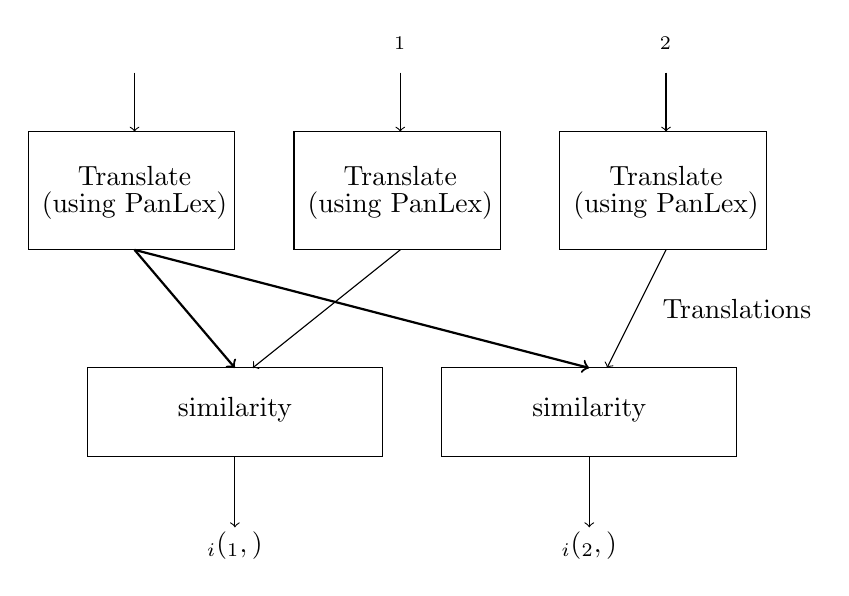
\begin{tikzpicture}[scale=0.75]

\node at (-4.2,3.5) {\MWE};
\node at (0.3,3.5) {$\component_{1}$};
\node at (4.8,3.5) {$\component_{2}$};

\draw [->,thin] (-4.2,3) -- (-4.2,2); 
\draw [->,thin] (0.3,3) -- (0.3,2); 
\draw [->,thin] (4.8,3) -- (4.8,2); 

\draw (-6,0) -- (-2.5,0) -- (-2.5,2) -- (-6,2) -- cycle;
\draw (-1.5,0) -- (2,0) -- (2,2) -- (-1.5,2) -- cycle;
\draw (3,0) -- (6.5,0) -- (6.5,2) -- (3,2) -- cycle;
\node at (-4.2,1.25) {Translate};
\node at (-4.2,0.75) {(using PanLex)};
\node at (0.3,1.25) {Translate};
\node at (0.3,0.75) {(using PanLex)};
\node at (4.8,1.25) {Translate};
\node at (4.8,0.75) {(using PanLex)};

\node at (6,-1) {Translations};

\draw [->,thick] (-4.2,0) -- (-2.5,-2); 
\draw [->,thick] (-4.2,0) -- (3.5,-2); 
\draw [->,thin] (0.3,0) -- (-2.2,-2); 
\draw [->,thin] (4.8,0) -- (3.8,-2); 


\draw (-5,-2) -- (0,-2) -- (0,-3.5) -- (-5,-3.5) -- cycle;
\draw (1,-2) -- (6,-2) -- (6,-3.5) -- (1,-3.5) -- cycle;
\node at (-2.5,-2.7) {similarity};
\node at (3.5,-2.7) {similarity};

\draw [->,thin] (-2.5,-3.5) -- (-2.5,-4.7); 
\draw [->,thin] (3.5,-3.5) -- (3.5,-4.7); 

\node at (-2.5,-5) {$\Sim_{i}(\component_{1},\MWE)$};
\node at (3.5,-5) {$\Sim_{i}(\component_{2},\MWE)$};

\end{tikzpicture}
\caption{\label{fig:diagram} Outline of our approach to computing the
  similarity of translations of an MWE with each of its component
  words, for a given target language. $\Sim_i$ is the similarity
  between the first or second component of the MWE, and the MWE
  itself, based on either string or distributional similarity, as
  measured using language $i$.}
\end{figure}



%\begin{figure}[t]
%
%\includegraphics[ width=\columnwidth]{Chapter4/schema1}
%\caption{
%\label{fig:ss:schema1}  Schematic outline of our proposed \isi{string similarity} approach using the $i$th target language}
%
%\end{figure}

\begin{figure}[t]

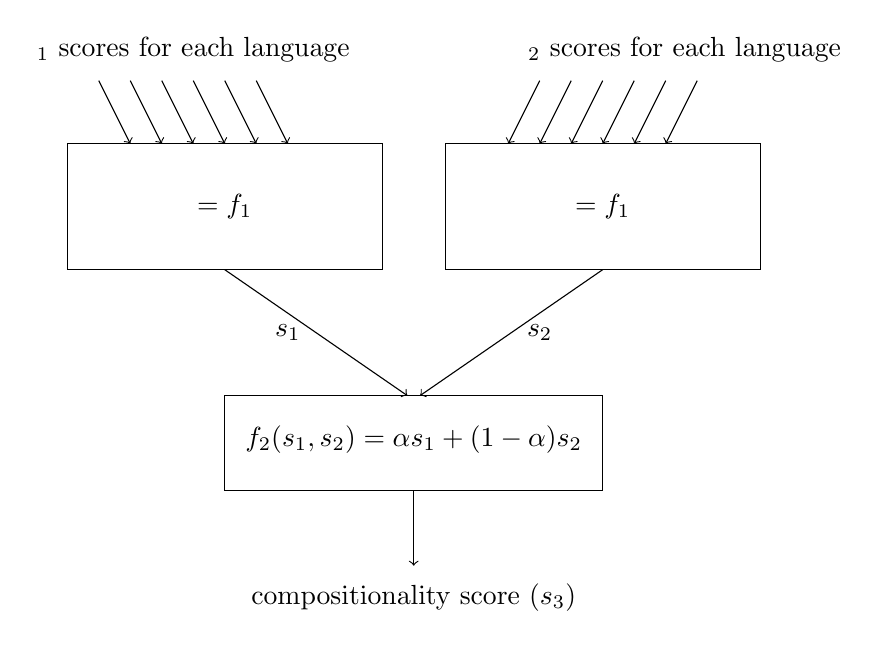
\begin{tikzpicture}[scale=0.80]


\node at (-3,3.5) {$\component_{1}$ scores for each language};
\node at (4.8,3.5) {$\component_{2}$ scores for each language};

\draw [->,thin] (-4.5,3) -- (-4,2); 
\draw [->,thin] (-4,3) -- (-3.5,2); 
\draw [->,thin] (-3.5,3) -- (-3,2); 
\draw [->,thin] (-3,3) -- (-2.5,2); 
\draw [->,thin] (-2.5,3) -- (-2,2); 
\draw [->,thin] (-2,3) -- (-1.5,2); 

\draw [->,thin] (5,3) -- (4.5,2); 
\draw [->,thin] (4.5,3) -- (4,2); 
\draw [->,thin] (4,3) -- (3.5,2); 
\draw [->,thin] (3.5,3) -- (3,2); 
\draw [->,thin] (3,3) -- (2.5,2); 
\draw [->,thin] (2.5,3) -- (2,2); 




\draw (-5,0) -- (0,0) -- (0,2) -- (-5,2) -- cycle;
\draw (1,0) -- (6,0) -- (6,2) -- (1,2) -- cycle;
\node at (-2.5,1) {$\Mean = f_1$};
\node at (3.5,1) {$\Mean = f_1$};

\node at (-1.5,-1) {$s_1$};
\node at (2.5,-1) {$s_2$};

\draw [->,thin] (-2.5,0) -- (0.4,-2); 
\draw [->,thin] (3.5,0) -- (0.6,-2); 


\draw (-2.5,-2) -- (3.5,-2) -- (3.5,-3.5) -- (-2.5,-3.5) -- cycle;

\node at (0.5,-2.7) {$f_{2}(s_1,s_2) = \alpha s_1 + (1-\alpha) s_2$};

\draw [->,thin] (.5,-3.5) -- (.5,-4.7); 

\node at (.5,-5.2) {compositionality score ($s_3$)};


\end{tikzpicture}
\caption{
\label{fig:diagram2}  Outline of the method for combining similarity scores
from multiple languages, across the components of the MWE.}

\end{figure}



%% Importantly, in order to make the method as
%% language-independent and broadly-applicable as possible, we make no
%% use of corpus preprocessing such as lemmatisation, and rely only on
%% the availability of a translation dictionary and monolingual corpora.

This chapter combines two previous works -- \cite{salehi2013} and
\cite{DBLP:conf/eacl/SalehiCB14} -- and extends them in the following ways:

%BS begin
\begin{compactitem}
\item two new \isi{string similarity} measures in
  \sectref{sec:ss:measures};
%% \item update of all results of \cite{salehi2013} in
%%   \sectref{sec:ss:results} in a way that it is now comparable to the
%%   results in \sectref{sec:distsim}. Previously, the results of
%%   \cite{salehi2013} and \cite{DBLP:conf/eacl/SalehiCB14} were not
%%   fully comparable as different folds were used.
\item updated results in \sectref{sec:ss:results} for the method of
  \cite{salehi2013} such that they are now comparable with the results
  of the method of \cite{DBLP:conf/eacl/SalehiCB14} in
  \sectref{sec:distsim} -- previously these results were not
  comparable because they used different cross-validation folds during
  evaluation;
\item new results for a dataset of \ili{German} noun compounds
  based on the \isi{string similarity} methods in \sectref{sec:ss:results};
\item additional error analysis in \sectref{sec:ss:erroranalysis} for
  \ili{English} verb-particle constructions;
\item two new translation-based similarity approaches, and results
  for these methods, in \sectref{sec:ch4-1:unsupervised};
\item experiments considering an alternative translation dictionary in
  \sectref{sec:dictcc};
\item analysis of the impact of window size on the distributional
  similarity approach in \sectref{sec:ds:calculating}.
\end{compactitem}
%BS end

\section{Related work}
\label{sec:RW}

%% TODO: Update RW section

Most recent work on predicting the compositionality\is{multiword expression!compositionality} of MWEs can be
divided into two categories: language/construction-specific and
general-purpose. This can be at either the token-level (over token
occurrences of an MWE in a corpus) or type-level (over the MWE string,
independent of usage). The bulk of work on compositionality\is{multiword expression!compositionality} has been
language/construction-specific and operated at the token-level, using
dedicated methods to identify instances of a given MWE, and specific
properties of the MWE in that language to predict compositionality\is{multiword expression!compositionality}
\citep{lin1999,kim2007,fazly-cook-stevenson:2009:CL}.

General-purpose token-level approaches such as \isi{distributional similarity}
have been commonly applied to infer the semantics of a word/MWE
\citep{Schone2001,Baldwin:2003,reddy2011a}. These techniques are based on
the assumption that the meaning of a word is predictable from its
context of use, via the neighbouring words of token-level
occurrences of the MWE. In order to predict the compositionality\is{multiword expression!compositionality} of a
given MWE using \isi{distributional similarity}, the different contexts of the
MWE are compared with the contexts of its components, and the MWE is
considered to be compositional if the MWE and component words occur in
similar contexts.

%bsalehi: many not be -> may not be
Identifying token instances of MWEs is not always easy, especially when
the component words do not occur sequentially. For example, consider
\localex{put on} in \localex{\textbf{put} your jacket \textbf{on}}, and
\localex{\textbf{put} your jacket \textbf{on} the chair}. In the first
example \localex{put on} is an MWE, while in the second example, \localex{put on}
is a simple verb with prepositional phrase and not an instance of an
MWE. Moreover, if we adopt a conservative identification method, the
number of token occurrences will be limited and the distributional
scores may not be reliable. Additionally, for morphologically-rich
languages, it can be difficult to predict the different word forms a
given MWE type will occur across, posing a challenge for our requirement
of no language-specific preprocessing.

\citet{pichotta2013} proposed a token-based method for identifying
\ili{English} phrasal verbs based on \isi{parallel corpora} for 50 languages. They
show that they can identify phrasal verbs better when they combine
information from multiple languages, in addition to the information
they get from a monolingual corpus. This finding lends weight to our
hypothesis that using translation data and \isi{distributional similarity}
from each of a range of target languages, can improve compositionality\is{multiword expression!compositionality}
prediction. Having said that, the general applicability of their
method is questionable -- there are many \isi{parallel corpora} involving
\ili{English}, but for other languages, this tends not to be the case.


In the literature, compositionality\is{multiword expression!compositionality} has been viewed as either
compositionality\is{multiword expression!compositionality} of the whole MWE as one unit
\citep{mccarthy2003,venkatapathy2005,Katz06automaticidentification,Biemann2011,farahmand2015},
or compositionality\is{multiword expression!compositionality} relative to each component
\citep{reddy2011a,hermann2012,SchulteImWalde+:2013}.  There have also
been studies which focus only on one component of the MWE.  For
example, \cite{korkontzelos2009} induce the most probable sense of an
MWE first, and then measure the semantic similarity between the MWE
and its semantic head.  This approach of considering only the head
component has been shown to be quite accurate for \ili{English} verb-particle 
constructions\is{verb-particle construction} \citep{bannard2003}. However, this might not
always be the case.  For example, as shown in \cite{reddy2011a}, the
compositionality\is{multiword expression!compositionality} of the first noun (the modifier) has more impact than
the second noun (the head) for \ili{English} noun compounds\is{noun compound}.

Elsewhere, a lot of work has been done on specific types of MWE in
specific languages.  In \ili{English}, studies have been done specifically
on VPCs \citep{mccarthy2003,bannard2003}, verb+noun MWEs
\citep{venkatapathy2005,mccarthy2007,fazly-cook-stevenson:2009:CL},
noun compounds\is{noun compound} \citep{reddy2011a}, and adjective+noun compounds
\citep{vecchi2011}.  There have also been studies focusing on a
specific language other than \ili{English}, such as Arabic \citep{saif2013}
and \ili{German} \citep{SchulteImWalde+:2013}. This chapter investigates
language independent approaches applicable to any type of MWE in any
language.


%% \citet{salehi2013} proposed a general-purpose type-based approach
%% using translation data from multiple languages, and \isi{string similarity}
%% between the MWE and each of the component words. They use training data
%% to identify the best-10 languages for a given family of MWEs, on which
%% to base the \isi{string similarity}, and once again find that translation data
%% improves their results substantially. Among the four \isi{string similarity}
%% measures they experimented with, longest common substring was found to
%% perform best. Their proposed method is general and applicable to
%% different families of MWEs in different languages. In this paper, we
%% reimplement the method of \citet{salehi2013} using longest common
%% substring (LCS), and both benchmark against this method and combine it
%% with our distributional similarity-based method.


\section{Resources}

In this section, we describe the datasets used to evaluate our method
and the \isi{multilingual dictionary} it requires. These are the same
resources as used by \cite{salehi2013} and
\cite{DBLP:conf/eacl/SalehiCB14}.

\subsection{Datasets}
\label{salehi:sec:dataset}

We evaluate our proposed method over three datasets (two \ili{English}, one
\ili{German}), as described below.

\subsubsection{English noun compounds (ENC)}
\label{sec:enc}

Our first dataset is made up of 90 binary \ili{English} noun compounds, from
the work of \citet{reddy2011a}. Each \isi{noun compound} was annotated by
multiple annotators using the integer scale 0 (fully
non-compositional) to 5 (fully compositional). A final
compositionality\is{multiword expression!compositionality} score was then calculated as the mean of the scores
from the annotators. If we simplistically consider 2.5 as the
threshold for compositionality\is{multiword expression!compositionality}, the dataset is relatively well
balanced, containing 48\% compositional and 52\% non-compositional
noun compounds. 

%BS begin
Spearman correlation was used to get an estimate of inter-annotator
agreement.  The average correlation for compound compositionality\is{multiword expression!compositionality} was
$\rho = 0.522$. This score was slightly higher for the compositionality\is{multiword expression!compositionality} of
components ($\rho = 0.570$ for the first component and $\rho = 0.616$ for the second
component).
%BS end

%% Following \citet{reddy2011a}, in combining the component-wise
%% distributional similarities for this dataset, we weight the first
%% component in \eqnref{eq:comp} higher than the second
%% ($\alpha=0.7$).



\subsubsection{English verb-particle constructions (EVPC)}
\label{sec:evpc}

The second dataset contains 160 \ili{English} verb-particle constructions
(VPCs), from the work of \citet{bannard2006}. In this dataset, a 
\isi{verb-particle construction} consists of a verb (the head) and a
prepositional particle (e.g.\ \localex{hand in}, \localex{look up} or
\localex{battle on}). For each component word (the verb and particle,
respectively), multiple annotators were asked whether the VPC entails
the component word. In order to translate the dataset into a
regression task, we calculate the overall compositionality\is{multiword expression!compositionality} as the
number of annotations of entailment for the verb, divided by the total
number of verb annotations for that VPC. That is, following
\citet{bannard2003}, we only consider the compositionality\is{multiword expression!compositionality} of the verb
component in our experiments.
%BS begin
The Kappa score between the multiple annotators is 0.372 for verb and
0.352 for the particle component.
 
%BS end
 %% (and as such $\alpha = 1$ in \eqnref{eq:comp}).

%% One area of particular interest with this dataset will be the
%% robustness of the method to function words (the particles), both
%% under translation and in terms of calculating distributional
%% similarity, although the findings of \citet{Baldwin:2006a} for
%% \ili{English} prepositions are at least encouraging in this
%% respect. Additionally, \ili{English} VPCs can occur in ``split'' form
%% (e.g.\ \localex{\textbf{put} your jacket \textbf{on}}, from our
%% earlier example), which will complicate \isi{identification}, and the
%% verb component will often be inflected and thus not match under our
%% \isi{identification} strategy (for both VPCs and the component verbs).



\subsubsection{German noun compounds (GNC)}

Our final dataset is made up of 246 \ili{German} noun compounds\is{noun compound}
\citep{von2009,SchulteImWalde+:2013}. Multiple annotators were asked to rate the
compositionality\is{multiword expression!compositionality} of each \ili{German} \isi{noun compound} on an integer scale of 1
(non-compositional) to 7 (compositional). The overall compositionality\is{multiword expression!compositionality}
score is then calculated as the mean across the annotators. Note that
the component words are provided as part of the dataset, and that
there is no need to perform decompounding. This dataset is significant 
%in being non-\ili{English}, and also in that 
as it is non-English and because of the fact that 
\ili{German} has relatively rich
morphology, which we expect to impact on the identification of both
the MWE and the component words.


\subsection{Multilingual dictionary\label{sec:multilingdict}}

To translate the MWEs and their components, we use PanLex
\citep{baldwin2010}. This online dictionary is massively multilingual,
covering more than 1353 languages\is{multilingual dictionary}. The translations are sourced from
handmade electronic dictionaries. It contains lemmatised words and
MWEs in a large variety of languages, with lemma-based (and less
frequently sense-based) links between them. 

For each MWE dataset (see \sectref{salehi:sec:dataset}), we translate each
MWE, and its component words, from the source language into many
target languages. These translations will be used in
\sectref{sec:stringsim} and \sectref{sec:distsim}. In instances where
there is no direct translation in a given language for a term, we use
a pivot language to find translation(s) in the target language. For
example, the \ili{English} \isi{noun compound} \localex{silver screen} has direct
translations in only 13 languages in PanLex, including Vietnamese
(\localex{m\`{a}n bac}) but not \ili{French}. There is, however, a
translation of \localex{m\`{a}n bac} into \ili{French}
(\localex{cin\'{e}ma}), allowing us to infer an indirect translation
between \localex{silver screen} and \localex{cin\'{e}ma}. In this way,
if there are no direct translations into a particular target language,
we search for a single-pivot translation via each of our other target
languages, and combine them all together as our set of translations
for the target language of interest.


\section{String similarity\label{sec:stringsim}}

In this section we present our string similarity-based method for
predicting compositionality\is{multiword expression!compositionality}, followed by experimental results using
this method. This section extends \cite{salehi2013} as described in
\sectref{salehi:sec:intro}.


\subsection{Compositionality prediction based on string similarity\label{sec:stringsimmethod}}

We hypothesize that compositional MWEs are more likely to be
word-for-word translations in a given language than non-compositional
MWEs. Hence, if we can locate the translations of the components in
the translation of the MWE, we can deduce that it is compositional.
As an example of our method, consider the \ili{English}-to-Persian\il{Farsi}
translation of \localex{kick the bucket} as a non-compositional MWE
and \localex{make a decision} as a semi-compositional MWE
(\tabref{translation-table}).\footnote{Note that the Persian
  words are transliterated into English for ease of understanding.} By
locating the translation of \localex{decision} (\localex{tasmim}) in
the translation of \localex{make a decision} (\localex{tasmim
  gereftan}), we can deduce that it is semi-compositional. However, we
cannot locate any of the component translations in the translation of
\localex{kick the bucket}. Therefore, we conclude that it is
non-compositional. Note that in this simple example, the match is
word-level, but that due to the effects of morphophonology, the more
likely situation is that the components don't match exactly (as we
observe in the case of \localex{khadamaat} and \localex{khedmat} for
the \localex{public service} example), which motivates our use of
\isi{string similarity} measures which can capture partial matches.

\begin{table}[t]

\begin{tabularx}{.8\textwidth}{XX}
\lsptoprule
English & Persian translation \\
\midrule
kick the bucket	& mord \\
kick	&zad \\
the 	&-- \\
bucket	&satl\\
\midrule
make a decision	& \textbf{tasmim} gereft\\
make	& sakht\\
a	&yek\\
decision	&\textbf{tasmim}\\
\midrule
public service & \localex{khadamaat} \textbf{omumi} \\
public &\textbf{omumi} \\
service & \localex{khedmat} \\
\lspbottomrule
\end{tabularx}

\caption{English MWEs and their components
  with their translation in Persian. Direct matches between the
  translation of an MWE and its components are shown in \textbf{bold};
  partial matches are shown in \localex{italics}.}
\label{translation-table}
\end{table}

\subsubsection{String similarity measures}
\label{sec:ss:measures}
We consider the following \isi{string similarity} measures to compare the
translations. In each case, we normalize the output value to the range
$[0,1]$, where 1 indicates identical strings and 0 indicates
completely different strings. We will indicate the translation of the
MWE in a particular language $t$ as $\MWE^t$, and the translation of a
given component in language $t$ as $\component^t$.

%% We consider longest common substring (LCS) as a measure to compare the
%% translations. The LCS output values are normalized to the range
%% $[0,1]$, where 1 indicates identical strings and 0 indicates
%% completely different strings. We will indicate the translation of the
%% MWE in a particular language $t$ as $\MWE^t$, and the translation of a
%% given component in language $t$ as $\component^t$.

\paragraph*{Longest common substring (LCS):}

The LCS measure finds the longest common substring between two
strings. For example, the LCS between \texttt{ABABC} and \texttt{BABCAB}
is \texttt{BABC}. We calculate a normalized similarity value based on
the length of the LCS as follows:
\begin{eqnarray}
\frac{\LCS(\MWE^t,\component^t)}{\min(\len(\MWE^t),\len(\component^t))}
\end{eqnarray}


\paragraph*{Levenshtein (LEV1):}
The Levenshtein distance calculates the number of basic edit
operations required to transform one word into the other. Edits
consist of single-letter insertions, deletions or substitutions. We
normalize LEV1 as follows:
\begin{eqnarray}
 1 - \frac{\LEVone(\MWE^t,\component^t)}{\max(\len(\MWE^t),\len(\component^t))}
\end{eqnarray}

 
\paragraph*{Levenshtein with substitution penalty (LEV2):}
One well-documented feature of Levenshtein distance
\citep{Baldwin:2009c} is that substitutions are in fact the
combination of an addition and a deletion, and as such can be
considered to be two edits. Based on this observation, we experiment
with a variant of LEV1 with this penalty applied for
substitutions. Similarly to LEV1, we normalize as follows:
\newpage 
\begin{eqnarray}
 1-  \frac{\LEVtwo(\MWE^t,\component^t)}{\len(\MWE^t)+\len(\component^t)}
\end{eqnarray}


\paragraph*{Smith Waterman (SW):}
This method is based on the Needleman-Wunsch algorithm,\footnote{The
 Needleman-Wunsch (NW) algorithm was designed to align two sequences
 of amino-acids \citep{needleman1970}. The algorithm looks for the
 sequence alignment which maximizes the similarity. As with the LEV
 score, NW minimizes edit distance, but also takes into account
 character-to-character similarity based on the relative distance
 between characters on the keyboard. We exclude this score because
 it is highly similar to the LEV scores and we did not obtain
 encouraging results using NW in our preliminary experiments.} and
was developed to locally-align two protein sequences
\citep{smith1981}. It finds the optimal similar regions by maximizing
the number of matches and minimizing the number of gaps necessary to
align the two sequences. For example, the optimal local sequence for
the two sequences below is \texttt{AT$--$ATCC}, in which
``\texttt{$-$}'' indicates a gap:
\begin{quote}
Seq1: \texttt{\textbf{ATGCATCC}CATGAC}\\
Seq2: \texttt{TCT\textbf{ATATCC}GT}
\end{quote}
As the example shows, it looks for the longest common string but has a
built-in mechanism for including gaps in the alignment (with
penalty). This characteristic of SW might be helpful in our task,
because there may be morphophonological variations between the MWE and
component translations (as seen above in the \localex{public service}
example). We normalize SW similarly to LCS:
\begin{eqnarray}
\frac{\len(\alignedSequence)}{\min(\len(\MWE^t),\len(\component^t))}
\end{eqnarray}
The aligned sequence is the combination of the common characters in the
optimal local sequence we found using SW. In the above example, the
aligned sequence is \texttt{ATATCC}.


%%BS begin

\paragraph*{Jaccard and Dice similarity:}
For further analysis, we experiment with Jaccard and Dice similarity,
which are well-known for measuring the similarity between two
sentences or bodies of text \citep{gomaa2013survey}.
%% CPC @BS Can we provide a citation to support this? 
%% BS done. This is the most relevant citation I could find
Both methods view the texts as sets of words, with similarity based on
the size of the intersection between the sets, but differ in the
way they are normalized. In our case, we expect relatively low overlap
at the word level due to morphophonology, and therefore calculate
Jaccard (J) and Dice (D) at the character- instead of word-level as
follows:

\begin{eqnarray}
J = {{|\MWE^t \cap \component^t|}\over{|\MWE^t| + |\component^t| - |\MWE^t \cap \component^t|}}
\end{eqnarray}


\begin{eqnarray}
D = \frac{2*| \MWE^t \cap \component^t |}{|\component^t | + | \MWE^t |}
\end{eqnarray}

%%BS end




\subsubsection{Calculating compositionality}
\label{sec:CM}

%% Given the scores calculated by LCS between the translations for a
Given the \isi{string similarity} scores calculated between the translations for a
given component word and the MWE, we need some way of combining scores
across component words. First, we measure the compositionality\is{multiword expression!compositionality} of each
component within the MWE ($s_1$ and $s_2$):
\begin{eqnarray}
  s_1 &=& f_{1}(\Sim_{1}(w_{1},\MWE),...,\Sim_{i}(w_{1},\MWE))\\
  s_2 &=& f_{1}(\Sim_{1}(w_{2},\MWE),...,\Sim_{i}(w_{2},\MWE))
\end{eqnarray}
where $\Sim$ is a similarity measure, $\Sim_{i}$ indicates that the
calculation is based on translations in language $i$, and $f_{1}$ is
a score combination function.

Then, we compute the overall compositionality\is{multiword expression!compositionality} of the MWE ($s_3$) from
$s_1$ and $s_2$ using $f_{2}$:
\begin{eqnarray}
  s_3 &=& f_{2}(s_{1},s_{2})
\end{eqnarray}
Since we often have multiple translations for a given component
word/MWE in PanLex, we exhaustively compute the similarity between
each MWE translation and component translation, and use the highest
similarity as the result of $\Sim_i$. If an instance does not have a
direct/indirect translation in PanLex, we assign a default value,
which is the mean of the highest and lowest annotation score for the
dataset under consideration. Note that word order is not an issue in
our method, as we calculate the similarity independently for each MWE
component.

We consider simple functions for $f_{1}$ such as mean, median,
product, minimum and maximum. $f_{2}$ was selected to be the same as $f_{1}$
in all situations, except when we use mean for $f_1$. Here, following
\citet{reddy2011a}, we experimented with weighted mean:
\newpage 
\begin{eqnarray}
f_{2}(s_1,s_2) = \alpha s_1 + (1-\alpha) s_2 
\end{eqnarray}
Based on 3-fold cross-validation, we chose $\alpha = 0.7$ for
\REDDY.\footnote{We considered values of $\alpha$ from 0 to 1,
  incremented by 0.1.} We found $\alpha = 0.7$ is also optimal for GNC.

Since we do not have judgements for the compositionality\is{multiword expression!compositionality} of the full VPC
in \BANNARD (we instead have separate judgements for the verb and
particle), we cannot use $f_{2}$ for this dataset. \citet{bannard2003}
observed that nearly all of the verb-compositional instances were also
annotated as particle-compositional by the annotators. In line with this
observation, we use $s_1$ (based on the verb) as the compositionality\is{multiword expression!compositionality}
score for the full VPC.


%% \begin{table}[t]
%% 
%% \begin{tabular}{l c l } \midrule
%% \multicolumn{3}{c}{NC}\\
%% Language&Frequency&Family\\
%% \midrule
%% \ili{Czech}&100&Slavic\\
%% Norwegian &100&Germanic\\
%% \ili{Portuguese} & 100 & Romance \\
%% Thai &99&Kam-thai\\
%% \ili{French} &95&Romance\\
%% Chinese&94&Chinese\\
%% Dutch &93&Germanic\\
%% \ili{Romanian} & 91 & Romance \\
%% Hindi  & 67 & Indic \\
%% Russian&43&Slavic\\
%%  \midrule

%% \end{tabular}

%% 
%% \caption{\label{bestLangNC-table} The 10 best languages for \REDDY using LCS.}
%% \end{table}

%% \begin{table}[t]
%% 
%% \begin{tabular}{lcl} \midrule
%% \multicolumn{3}{c}{VPC:verb}\\
%% Language&Frequency&Family\\
%% \midrule
%% Basque &100 & Basque \\
%% \ili{Lithuanian} &100&Baltic \\
%% Slovenian &100&Slavic \\
%% \ili{Hebrew} &99&Semitic\\
%% Arabic &98&Semitic\\
%% \ili{Czech}	&95 & Slavic\\
%% Slovak &92&Slavic\\
%% Latin	& 79 & Italic \\
%% Tagalog	& 74 & Austronesian \\
%% \ili{Polish} & 44 & Slavic \\
%%  \midrule

%% \end{tabular}
%% 
%% \caption{\label{bestLangVPC-table} The 10 best languages for the verb
%%   component of \BANNARD using LCS.}
%% \end{table}


%% \begin{table}[t]
%% 
%% \begin{tabular}{ l c l} \midrule
%% \multicolumn{3}{c}{VPC:particle}\\
%% Language&Frequency&Family\\
%% \midrule
%% \ili{French} &100&Romance\\
%% Icelandic &100	&Germanic\\
%% Thai &100&Kam-thai\\
%% Indonesian &92&Indonesian\\
%% \ili{Spanish} &90 &Romance\\
%% Tamil	&87 & Dravidian\\
%% \ili{Turkish}	&83&Turkic\\
%% Catalan & 79 & Romance\\
%% Occitan	& 76 & Romance\\
%% \ili{Romanian}	& 69 & Romance \\
%%  \midrule
%% \end{tabular}
%% 
%% \caption{The 10 best languages for the particle component of \BANNARD
%%   using LCS.}
%% \label{bestLangVPCparticle-table} 
%% \end{table}


\subsubsection{Language selection\label{sec:ss-lang-selection}}

Our method is based on the translation of an MWE into many
languages. First, we chose 54 languages for which
relatively large corpora were available.\footnote{In
  \sectref{sec:distsim} these corpora will be used to compute
  \isi{distributional similarity}. Note that the \isi{string similarity} methods of interest here do not rely on the
  availability of large corpora.} The coverage, or the number of
instances which have direct/indirect translations in PanLex, varies
from one language to another. In preliminary experiments, we noticed
that there is a high correlation (between roughly $r = 0.6$ and 0.8 across
the three datasets) between the usefulness of a language and its
translation coverage on MWEs. Therefore, we excluded languages with
MWE translation coverage of less than 50\%. Based on nested 10-fold
cross-validation in our experiments, we select the 10 most useful
languages for each cross-validation training partition, based on the
Pearson correlation between the given scores in that language and
human judgements.\footnote{Note that for VPCs, we calculate the
  compositionality of only the verb part, because we don't have the
  human judgements for the whole VPC.}  The 10 best languages are
selected based only on the training set for each fold. (The languages
selected for each fold will later be used to predict the
compositionality\is{multiword expression!compositionality} of the items in the testing portion for that fold.)

%% In \localtabref[s]{bestLangNC-table}, \ref{bestLangVPC-table} and
%% \ref{bestLangVPCparticle-table}, we show how often each language was
%% selected in the top-10 languages over the combined 100 (10$\times$10)
%% folds of nested 10-fold cross validation, based on LCS.\footnote{Since
%%   our later results show that LCS and SW have higher results, we only
%%   show the best languages using LCS. These largely coincide with those
%%   for SW.}  The tables show that the selected languages were mostly
%% consistent over the folds. The languages are a mixture of Romance,
%% Germanic and languages from other families (based on
%% \citet{voegelin1977}), with no standout language which performs well
%% in all cases (indeed, no language occurs in all three
%% tables). Additionally, there is nothing in common between the verb and
%% the particle top-10 languages.



\subsection{Results\label{sec:ss:results}}


%% \begin{table}[t]
%% 
%% \smaller
%% \begin{tabular}{cccccccccccccc}
%% \toprule
%% & \multicolumn{3}{c}{ENC} && \multicolumn{2}{c}{EVPC} && \multicolumn{3}{c}{GNC}\\
%%   \cmidrule{2-4}
%%   \cmidrule{6-7}
%%   \cmidrule{9-11}
%% &  N1 & N2 & NC && Verb & Particle && N1 & N2 & NC  \\
%% \midrule
%%   LCS  & 0.523 & \textbf{0.436} & \textbf{0.644}  &&\textbf{0.385}  & \textbf{0.509}	&& 0.358  &  \textbf{0.357}   & 0.372\\
%% DS &&& 0.700 &&0.177& &&&&0.141\\
%% \bottomrule
%% \end{tabular}
%% 
%% \caption{\label{tab:stringsimresults} Correlation on each dataset. N1, N2,
%%   and NC, are the first component of the \isi{noun compound}, its second
%%   component, and the \isi{noun compound} itself, respectively, for ENC and
%%   GNC. DS stands for distributional similarity}
%% \end{table}

\begin{table}[t]

\begin{tabular}{lccc}
\lsptoprule
Method  & ENC   & EVPC  & GNC   \\
\midrule
SW   & \textbf{0.644} & 0.349 & 0.379 \\
LCS  & \textbf{0.644} & \textbf{0.385} & 0.372 \\
LEV1 & 0.502 & 0.328 & 0.318 \\
LEV2 & 0.566 & 0.327 & \textbf{0.389} \\
Jaccard& 0.474 & 0.335 & 0.299\\
Dice & 0.557 & 0.331 & 0.370\\
\midrule
Unsupervised (family) & 0.556 & 0.257 & 0.164 \\
Unsupervised (coverage) & 0.642 & 0.323 & 0.343 \\
\lspbottomrule
\end{tabular}
\caption{Correlation ($r$) on each dataset, for
  each string similarity measure. The best correlation for each
  dataset is shown in boldface.}
\label{tab:stringsimresults}

\end{table}

As mentioned above, we perform nested 10-fold cross-validation to
select the 10 best languages on the training data for each fold. The
selected languages for a given fold are then used to compute $s_1$ and
$s_2$ (and $s_3$ for NCs) for each instance in the test set for that
fold.  The scores are compared with human judgements using Pearson's
correlation.  

We experimented with five functions for $f_1$, namely mean, median,
product, maximum and minimum. Among these functions, mean performed
consistently better than the others, and as such we only present results
using mean in \tabref{tab:stringsimresults}.

%% Besides LCS, we experimented with three other \isi{string similarity}
%% measures, namely levenshtein,\footnote{calculates for the number of
%%   basic edit operations required to transpose one word into the
%%   other. Edits consist of single-letter insertions, deletions or
%%   substitutions.} levenshtein with substitution
%% penalty, \footnote{substitution is considered to be two edits
%%   \citep{Baldwin:2009c}.}  and Smith-Waterman (SW)
%% \citep{smith1981}.\footnote{SW looks for the longest common string but
%%   has an in-built mechanism for including gaps in the alignment (with
%%   penalty). This characteristic of SW might be helpful in our task,
%%   because there may be morphophonological variations between the MWE
%%   and component translations (as seen above in the \localex{public
%%     service} example }

%% For the most part, LCS and SW perform better than the other measures.
%% There is little to separate these two methods, partly because they both
%% look for a sequence of similar characters, unlike LEV1 and LEV2 which do
%% not consider contiguity of match. The results showing the best performing 
%% combination, which is Mean for $f_1$ and LCS for $f_2$, are shown in
%% \localtabref{tab:stringsimresults}. 

For ENC, LCS and SW perform best, while for EVPC, LCS performs best
with SW being the next best measure. Both LCS and
SW look for a sequence of similar characters, unlike LEV1 and LEV2, 
which are not affected by match contiguity. For GNC, LEV2, SW and LCS
perform better than LEV1. However, unlike the other two datasets, LEV2
is the best performing method, and SW is slightly better than LCS.

%%BS begin
For all datasets, Jaccard and Dice perform worse than SW and LCS. This
shows that, despite being useful in measuring the similarity between
sentences, these two measures do not perform well in this
compositionality\is{multiword expression!compositionality} prediction task. The relatively poor performance of
these measures could be because, unlike the other measures, Jaccard and
Dice are calculated independently of the order of characters. Dice
performs better than Jaccard for ENC and GNC, while Jaccard performs
slightly better than Dice for EVPC. 

%%BS End

The results support our hypothesis that using multiple target
languages rather than one, results in a more accurate prediction of
MWE compositionality\is{multiword expression!compositionality}. Our best result using the 10 selected languages
on \REDDY is $r = 0.644$, as compared to the best single-language
correlation of $r = 0.543$ for \ili{Portuguese}. On \BANNARD, the best LCS result
for the verb component is $r = 0.385$, as compared to the best
single-language correlation of $r = 0.342$ for \ili{Lithuanian}. For GNC, the best
correlation of $r = 0.389$ is well above the highest correlation of a single
language of roughly $r = 0.32$.

In \sectref{sec:distsim} we will combine this \isi{string similarity}
approach with an approach based on \isi{distributional similarity}, and
compare it against a baseline and state-of-the-art approaches.

%% bsalehi: added below text
%% On GNC, as for the ENC and EVPC datasets, Mean is the best $f_1$ function. 
%% LEV2, SW and LCS are performing better than LEV1. Unlike the other two datasets, 
%% LEV2 is the best performing method and SW is slightly better than LCS. 

%% Distributional similarity approach is considered as the baseline,
%% which requires identifying the instances in a large corpus. \ili{German} is
%% a morphologically-rich language, with marking of number and case on
%% nouns. Given that we do not perform any lemmatisation or other
%% language-specific preprocessing, we inevitably achieve low recall for
%% the \isi{identification} of \isi{noun compound} tokens, although the precision
%% should be nearly 100\%. Partly because of the resultant sparseness of
%% semantic vectors \footnote{Due to morphological richness} in the
%% \isi{distributional similarity} method, the result for DS is low ($r$ =
%% 0.141) for GNC.  Simple \isi{string similarity} achieves better results for
%% this dataset.


%% Finally, we experimented with combining our method
%% (\textsc{StringSim$_{\textsc{mean}}$}) with a reimplementation of
%% the method of \citet{reddy2011a}, based on simple averaging, as
%% detailed in \localtabref{tab:usReddy}. The results are higher than
%% both component methods and the state-of-the-art for \REDDY,
%% demonstrating the complementarity between our proposed method and
%% methods based on \isi{distributional similarity}.


%% \begin{table}[t]
%% 
%% \begin{tabular}{l c c}
%% $sim()$& \textsc{StringSim$_{\textsc{mean}}$} & \textsc{StringSim$_{\textsc{mean}}$} + Reddy et al.\\ \midrule
%% SW & 0.637 & 0.735 \\
%% LCS & \textbf{0.649} & \textbf{0.742} \\
%% LEV1 & 0.523 & 0.724 \\
%% LEV2& 0.577 & 0.726
%% \\ \midrule

%% \end{tabular}
%% %bsalehi: caption updated
%% \caption{\label{tab:usReddy} Correlation after combining Reddy et
%%   al.'s method and our method with Mean for $f_{1}$
%%   (\textsc{StringSim$_{\textsc{mean}}$}).  The correlation using Reddy
%%   et al.'s method is 0.714.}
%% 
%% \end{table}

%% \begin{table}[t]
%% 
%% \begin{tabular}{l c c c c}
%% Method & Precision & Recall & F-score ($\beta=1$) & Accuracy \\ \midrule
%% \citet{bannard2003} & 0.608 & 0.666 & 0.636 & 0.600 \\
%% \textsc{StringSim$_{\textsc{mean}}$} &  0.862 & 0.718 & 0.774 & 0.693 \\ \midrule
%% \end{tabular}
%% \caption{\label{VPCcompare-table} Results for the classification
%%   task. \textsc{StringSim$_{\textsc{mean}}$} is our method using Mean for
%%   $f_{1}$}
%% 
%% \end{table}


%% \begin{table}[t]
%% 
%% \begin{tabular}{l c c@{\hspace{2em}} c} 
%% \toprule
%% Dataset &   Supervised LCS && Unsupervised LCS \\ \midrule
%% % & First component & Second component  & MWE & MWE+DS \\\midrule
%% ENC  & 0.644 && 0.642 \\
%% %0.523 & 0.436 & 0.644 & 0.739\\
%% %&Unsupervised & 0.642&& 0.740 \\ \midrule
%% %0.440 & 0.268 & 0.555 & 0.716\\\midrule
%% EVPC& 0.385 && 0.323 \\
%% %0.385 & 0.509 & 0.385 & 0.360\\
%% %&Unsupervised & 0.323 && 0.318 \\ \midrule %put the wright number instead of 0.318
%% %0.334 & 0.447 & 0.334 & 0.318\\\midrule
%% GNC & 0.372 && 0.343\\
%% %0.358 & 0.357 & 0.372 & 0.353\\
%% %&Unsupervised & 0.343 && 0.332 \\
%% % 0.256 & 0.252 & 0.265 & 0.253\\\midrule
%% \bottomrule
%% \end{tabular}
%% \caption{\label{tab:ss:unsupervised} Correlation on ENC, EVPC and GNC datasets using supervised and unsupervised string similarity approach.}
%% 
%% \end{table}

\subsubsection{Error analysis}
\label{sec:ss:erroranalysis}

We analysed items in \REDDY which have a high absolute difference (more than
2.5) between the human annotation and our scores (using LCS and
mean). The words are \localex{cutting edge}, \localex{melting pot},
\localex{gold mine} and \localex{ivory tower}, which are
non-compositional according to \REDDY. After investigating their
translations, we came to the conclusion that the first three MWEs have
word-for-word translations in most languages. Hence, they disagree
with our hypothesis that word-for-word translation is a strong
indicator of compositionality\is{multiword expression!compositionality}.  The word-for-word translations might
be because of the fact that they have both compositional and
non-compositional senses, or because they are calques (loan
translations). However, we have tried to avoid such problems with
calques by using translations into several languages.

For \localex{ivory tower} (``a state of mind that is discussed as if it
were a place'')\footnote{This definition is from Wordnet 3.1.} we
noticed that we have a direct translation into 13 languages. Other
languages have indirect translations. By checking the direct
translations, we noticed that, in \ili{French}, the MWE is translated to
\localex{tour} and \localex{tour d'ivoire}. A noisy (wrong) translation of
\localex{tour} \gl{tower} resulted in wrong indirect translations for
\localex{ivory tower} and an inflated estimate of compositionality\is{multiword expression!compositionality}.

We repeat the same error analysis for the EVPC dataset. The items with
a high difference between the human annotation and our scores are:
\localex{carry out}, \localex{drop out}, \localex{get in},
\localex{carry away}, \localex{wear down} and \localex{turn on}. All
of these items are annotated as non-compositional. These VPCs also
have a compositional sense beside the non-compositional meaning. Also,
as with the ENC dataset, we have problems of calques. For example, 
\localex{drop out} when translated to \ili{German} (\localex{ausfallen})
includes the word \localex{fallen}, which is one of the translations of
\localex{drop}.

\subsubsection{Unsupervised approach}
\label{sec:ch4-1:unsupervised}
%%BS begin


The proposed translation-based \isi{string similarity} approach has been
supervised so far, in that the best target languages are selected
based on training data. In this section, we propose two unsupervised
approaches in which: (1) only the target languages of the same language
family as the source language are considered; and (2) only the 10
target languages with the highest translation coverage are considered.

\paragraph*{Languages of the same family:}

%% TODO Can we provide a citation or better argument to support trying
%% this approach?

We hypothesize that translations into target languages in the same
language family as the source language might be particularly useful
for compositionality\is{multiword expression!compositionality} prediction for MWEs in the source language. To
test this hypothesis, we consider an unsupervised approach in which
only languages in the same family as the source language are used when
computing the compositionality\is{multiword expression!compositionality} scores.

In this unsupervised approach, LCS scores of the languages of the same
family as the source language (here Germanic, for both the \ili{English} and
\ili{German} datasets) are considered. The Germanic languages among our 54
languages are: \ili{English}, \ili{German}, \ili{Danish}, \ili{Dutch}, \ili{Icelandic},
\ili{Luxembourgish}, \ili{Norwegian} and \ili{Swedish}.

Results for this unsupervised approach are shown in
\tabref{tab:stringsimresults} (``Unsupervised (family)''). This
approach performs substantially worse than the corresponding
supervised approach based on LCS, for each dataset. This drop in
performance could be because almost none of the 10 best languages
selected in the supervised approach are in the same language family as
the source language. The shared languages between the supervised approach
and this approach are Dutch and Norwegian for ENC, \ili{English} for GNC. 
There is no shared language between the two approaches when using EVPC.

%% CPC @BS Which languages are shared between the supervised approach
%% with LCS and this unsupervised approach. I.e., Can we clarify what
%% ``almost'' means above.
%% BS: added above

%% The results of our unsupervised approach along with the supervised
%% approach are shown in Table \ref{tab:ss:unsupervised} for the three
%% datasets.  
\paragraph*{Languages with the highest translation coverage:}

In the proposed supervised setup, the best target languages are those
whose scores have the highest correlation with gold-standard
annotations.  According to our experiments, we showed that there is a
strong correlation between being a good language for this
compositionality\is{multiword expression!compositionality} prediction task and its coverage in PanLex (in the
range of roughly $0.6 < r < 0.8$ across the three datasets). In other words, the
target languages to which most of the source language MWEs have a
translation in PanLex, result in higher correlation for
compositionality\is{multiword expression!compositionality} prediction.

We now consider an unsupervised approach, in which only the 10
target languages with the highest translation coverage are
considered. The results of this unsupervised approach, again using
LCS, are shown in \tabref{tab:stringsimresults} (``Unsupervised
(coverage)''). According to the results, despite the lower correlation
scores for the proposed unsupervised method, this method is comparable
to the supervised approach.  Therefore, in the case of not having a
training set for a group of MWEs (no matter in what language or what
type of MWE), we suggest using the target languages to which the
majority of those MWEs have a translation.

The 10 languages with highest correlation for ENC, EVPC and GNC are
shown in \tabref{tab:ss:cov}. There is some overlap between the
list of languages with the highest coverage and the 10 best languages
selected in our supervised approach, as shown in boldface for each
dataset.


\begin{table}[t]

\begin{tabularx}{.8\textwidth}{XXX } \lsptoprule

ENC&EVPC&GNC\\
\midrule
German & German & \textbf{English}\\
Finnish  & Finnish & Japanese\\
\textbf{French}& French & French\\
Italian& Italian & Italian\\
Russian&  Japanese & Russian\\
Spanish & Hungarian & Hungarian\\
\textbf{Portuguese} & Dutch & Dutch\\
Japanese& \textbf{Polish}&  Turkish\\
\textbf{Chinese} & Chinese & Chinese\\
\textbf{Czech}&  \textbf{Czech} &\textbf{Czech}\\
\lspbottomrule

\end{tabularx}


\caption{\label{tab:ss:cov} The 10 languages with the highest
  translation coverage for ENC, EVPC and GNC. Languages also selected
  by the supervised approach are shown in \textbf{boldface}.}
\end{table}



%%BS end

\section{An alternative multilingual dictionary\label{sec:dictcc}}
\largerpage[2]
In this section we consider the same string similarity-based approach
to predicting compositionality\is{multiword expression!compositionality} as in \sectref{sec:stringsimmethod}, but
using an alternative \isi{multilingual dictionary} to PanLex, specifically
\dictcc.\footnote{\url{https://www.dict.cc/}}

%% \subsection{What is \dictcc}

\begin{table}[t]


\begin{tabularx}{.8\textwidth}{XXccc}
\lsptoprule
Dictionary & Method  & ENC   & EVPC  & GNC   \\
\midrule
\dictcc \\
\midrule
&SW   & .269 & .217 & .514 \\
&LCS  & .251 & .262 & \textbf{.523} \\
&LEV1 & .181 & .161 & .482 \\
&LEV2 & .163 & .189 & .474 \\
&Jaccard& .158 & .127 & .442 \\
&Dice & .230 & .192 & .420 \\
\midrule
PanLex \\
\midrule
&SW   & \textbf{.559} & \textbf{.294} & .270 \\
&LCS  & .551 & .276 & .290 \\
&LEV1 & .388 & .274 & .276 \\
&LEV2 & .512 & .281 & .262 \\
&Jaccard& .459 & .241 & .267 \\
&Dice & .541 & .235 & .197 \\
\lspbottomrule
\end{tabularx}
\caption{Correlation ($r$) on each dataset, for each string similarity
  measure, using \dictcc and PanLex as the translation dictionary. The
  best correlation for each dataset is shown in boldface.}
\label{tab:stringsimresults-ccdict}

\end{table}

\dictcc is a translation dictionary that provides translations for
both \ili{English} and \ili{German} into 26 languages spoken in Europe. It is a
crowd-sourced dictionary, with translations being contributed, and
refined, by users. Due to the relatively small number of languages it
covers, relying on \dictcc goes against our goals of developing
compositionality\is{multiword expression!compositionality} prediction methods that are applicable to any
language; we could not use \dictcc to predict the compositionality\is{multiword expression!compositionality} of,
for example, a \ili{French} MWE, because translations are not available for
\ili{French} into many languages (only \ili{English} and \ili{German}). Nevertheless, by
considering the use of an alternative translation dictionary (which is
applicable to the \ili{English} and \ili{German} datasets we use for evaluation)
we can learn whether our approach to predicting compositionality\is{multiword expression!compositionality}
implicitly relies on information particular to PanLex, or whether an
alternative dictionary can be substituted in its place.

We chose target languages available in \dictcc that overlap with the
set of 54 target languages used in experiments with PanLex in
\sectref{sec:stringsimmethod}. This resulted in 22 target
languages. We introduced this restriction, as opposed to using all
languages available in \dictcc, to allow us to compare PanLex and
\dictcc when using the exact same set of target languages.


Results for the string similarity-based approach to predicting
compositionality\is{multiword expression!compositionality}, using \dictcc and PanLex, each with the same 22
target languages, are shown in
\tabref{tab:stringsimresults-ccdict}. The 10 best languages are
selected using the same method as in \sectref{sec:ss-lang-selection}.

%% \subsection{results}



For each translation dictionary and dataset, the best method is always
one of either SW or LCS, and in many cases these are the top two
methods (with the exceptions being EVPC and GNC using PanLex). These
methods were also found to perform well in \sectref{sec:ss:results}
when using PanLex and 54 target languages. This demonstrates that the 
methods are robust to the choice of specific translation dictionary,
and when the number of target languages is substantially reduced.

\begin{figure}[t]

  \includegraphics[width=0.75\textwidth]{figures/coverage-boxplot.pdf}
\caption{Boxplots showing the percentage of expressions in each
  dataset covered by \dictcc and PanLex, over the 22 target
  languages.\label{fig:ccdict:coverage}}

\end{figure}

There are, however, substantial differences between the results using
different translation dictionaries. For any combination of dataset and
method, the results using PanLex are always better than those using
\dictcc for ENC and EVPC, while for GNC, the results using \dictcc are
always better. To understand why this is the case, for each dataset 
and dictionary, and for each of the 22 target languages, we computed the 
proportion of expressions for which translations are
available. Boxplots illustrating these findings are shown in
\figref{fig:ccdict:coverage}. On average across the target languages,
many more expressions are covered by PanLex than \dictcc for ENC and
EVPC, while for GNC the coverage is higher for \dictcc. For example,
according to \figref{fig:ccdict:coverage}, for EVPC the coverage for
almost all of the 22 target languages is close to 100\% in PanLex.

Because it in keeping with our goal of building methods for
compositionality\is{multiword expression!compositionality} prediction that are applicable to any language, and
because it gives the best results in two out of three cases for the
datasets used for evaluation, we will only consider PanLex as the
translation dictionary for the remainder of this chapter.


\section{Distributional similarity\label{sec:distsim}}

In this section we describe a method for predicting compositionality\is{multiword expression!compositionality}
based on the same framework as in \sectref{sec:stringsim}, but using
\isi{distributional similarity} instead of \isi{string similarity}. This section
extends \cite{DBLP:conf/eacl/SalehiCB14} as described in
\sectref{salehi:sec:intro}.

\subsection{Compositionality prediction based on distributional similarity\label{sec:distsimmodel}}

To predict the compositionality\is{multiword expression!compositionality} of a given MWE, we first measure the
semantic similarity between the MWE and each of its component words
using \isi{distributional similarity} based on a monolingual corpus in the
source language.  We then repeat the process for translations of the
MWE and its component words into each of a range of target languages,
calculating \isi{distributional similarity} using a monolingual corpus in
the target language. We additionally use supervised learning to
identify which target languages (or what weights for each language)
optimise the prediction of compositionality\is{multiword expression!compositionality}. We hypothesise that by
using multiple translations -- rather than only information from the
source language -- we will be able to better predict
compositionality\is{multiword expression!compositionality}. We further optionally combine our proposed approach
with the LCS-based \isi{string similarity} method from
\sectref{sec:stringsim}.

Below, we detail our method for calculating \isi{distributional similarity}
in a given language, the different methods for combining similarity
scores into a single estimate of compositionality\is{multiword expression!compositionality}, and finally the
method for selecting the target languages to use in calculating
compositionality\is{multiword expression!compositionality}.


\subsubsection{Calculating distributional similarity\label{sec:ds:calculating}}

We collected monolingual corpora for each of the 52 languages (51 target
languages + 1 source language) from XML dumps of Wikipedia. These
languages are based on the 54 target languages used in
\sectref{sec:stringsim}, excluding \ili{Spanish} because we happened not to
have a dump of \ili{Spanish} Wikipedia, and also Chinese and Japanese
because of the need for a language-specific word tokeniser. The raw
corpora were preprocessed using the WP2TXT
toolbox\footnote{\smaller\url{http://wp2txt.rubyforge.org/}} to
eliminate XML tags, HTML tags and hyperlinks, and then tokenisation
based on whitespace and punctuation was performed. The corpora vary in
size from roughly 750M tokens for \ili{English}, to roughly 640K tokens for
Marathi.

In order to be consistent across all languages and to be as
language-indepen\-dent as possible, we calculate distributional
similarity\is{distributional similarity!language-independent measure} in the following manner for a given language.

Tokenisation is based on whitespace delimiters and punctuation; no
lemmatisation or case-folding is carried out. Token instances of a
given MWE or component word are identified by full-token $n$-gram
matching over the token stream. We assume that all full stops and
equivalent characters for other orthographies are sentence boundaries,
and chunk the corpora into (pseudo-)sentences on the basis of
them. For each language, we identify the 51st--1050th most frequent
words, and consider them to be content-bearing words, in the manner of
\citet{Schutze:1997}. This is based on the assumption that the top-50
most frequent words are stop words, and not a good choice of word for
calculating \isi{distributional similarity} over. That is not to say that we
can't calculate the \isi{distributional similarity} for stop words, however
(as we will for the EVPC dataset) they are simply not used as the
dimensions in our calculation of \isi{distributional similarity}.

\begin{table}[t]

\begin{tabular}{l c} 
\lsptoprule
Context window &Correlation ($r$) \\\midrule
Sentence & 0.425 \\
Window ($N$=3) & 0.175 \\
Window ($N$=3, with positional index) & 0.031 \\
\lspbottomrule
\end{tabular}
\caption{\label{tab:ds:premResult} Results of distributional similarities using 10 best languages on ENC dataset ($N$ is window size)}

\end{table}


We form a vector of content-bearing words across all token occurrences
of the target word, on the basis of these 1000 content-bearing words. Our
preliminary results on selecting the best context window size are
shown in \tabref{tab:ds:premResult}. According to this table, for
predicting the compositionality\is{multiword expression!compositionality} using the best 10 languages, the
sentence context window results in a higher correlation. We use
sentence boundaries as the context window in the rest of our
experiments. According to \citet{weeds2003} and
\citet{Pado:Lapata:2007}, using dependency relations with the
neighbouring words of the target word can better predict the meaning
of the target word. However, in line with our assumption of no
language-specific preprocessing, we just use word
co-occurrence. Finally, \isi{distributional similarity} is calculated over
these context vectors using cosine similarity.

\subsubsection{Calculating compositionality}
\label{sec:computing-compositionality}
The procedure of calculating the compositionality\is{multiword expression!compositionality} is similar to what
we used in \sectref{sec:CM}: after translating the MWE and its
components into multiple languages and measuring the distributional
similarity between the translations of the MWE and its components
(\figref{fig:diagram}), we find the best languages according to the
training set. Then, we combine the scores from those best languages
and finally calculate a combined compositionality\is{multiword expression!compositionality} score from the
individual distributional similarities between each component word and
the MWE. Based on our findings in \sectref{sec:CM}, we combine the
component scores using the weighted mean (\figref{fig:diagram2}):

\begin{equation}
  \text{Compositionality} = \alpha s_{1} + (1-\alpha) s_{2}
  \label{eq:comp}
\end{equation} 
where $s_{1}$ and $s_{2}$ are the scores for the first and the second
component, respectively. We use different $\alpha$ settings for each
dataset, based on the settings from \sectref{sec:CM}.

We experiment with a range of methods for calculating
compositionality\is{multiword expression!compositionality}, as follows:
\begin{description}
\item[\CSsource:] calculate \isi{distributional similarity} using only
  \isi{distributional similarity} in the source language corpus. (This is
  the approach used by \citet{reddy2011a}, as discussed in \sectref{sec:RW}.)
\item[\CStarg:] exclude the source language and compute the mean of
  the \isi{distributional similarity} scores for the best-$N$ target
  languages. The value of $N$ is selected according to training data,
  as detailed in \sectref{sec:lang-selection}.\footnote{In the case
    that no translation (direct or indirect) can be found for a given
    source language term into a particular target language, the
    compositionality\is{multiword expression!compositionality} score for that target language is set to the
    average across all target languages for which scores can be
    calculated for the given term. If no translations are available
    for any target language (e.g.\ the term is not in PanLex) the
    compositionality\is{multiword expression!compositionality} score for each target language is set to the
    average score for that target language across all other source
    language terms.}
\item[\CSsourcetarg:] calculate \isi{distributional similarity} over both the
  source language (\CSsource) and the mean of the best-$N$ languages
  (\CStarg), and combine via the arithmetic mean.\footnote{We also
    experimented with taking the mean over all the languages -- target
    and source -- but found it best to combine the scores for the
    target languages first, to give more weight to the source language.}
  This is to examine the hypothesis that using multiple target languages
  is better than just using the source language.
\item[\CSsvr:] train a support vector regressor (SVR:
  \citet{Smola:Scholkopf:2004}) over the distributional similarities
  for all 52 languages (source and target languages).
\item[\CSstring:] calculate \isi{string similarity} using the LCS-based method
  of \sectref{sec:stringsim}. 
	%BS begin
	LCS is chosen because, in general, it performs better than 
	the other \isi{string similarity} measures.
	%Bs end
\item[\CSstringDS:] calculate the mean of the \isi{string similarity} (\CSstring)
  and \isi{distributional similarity} in the source language.
\item[\CSall:] calculate the mean of the \isi{string similarity} (\CSstring)
  and \isi{distributional similarity} scores (\CSsource and \CStarg).
\end{description}



\subsubsection{Selecting target languages}
\label{sec:lang-selection}

We experiment with two approaches for combining the compositionality\is{multiword expression!compositionality}
scores from multiple target languages.

First, in \CStarg (and \CSsourcetarg and \CSall that build off it),
following the approach from \sectref{sec:ss-lang-selection}, we use
training data to rank the target languages according to Pearson's
correlation between the predicted compositionality\is{multiword expression!compositionality} scores and the
gold-standard compositionality\is{multiword expression!compositionality} judgements. However, in this case,
based on this ranking, we take the best-$N$ languages (instead of the
best-10 languages as in \sectref{sec:ss-lang-selection}) and again
combine the individual compositionality\is{multiword expression!compositionality} scores by taking the
arithmetic mean. We select $N$ by determining the value that optimises
the correlation over the training data. In other words, the selection
of $N$ and accordingly the best-$N$ languages are based on nested
cross-validation over training data, independently of the test data
for that iteration of cross-validation.

Second in \CSsvr, we take the compositionality\is{multiword expression!compositionality} scores from the
source and all 51 target languages, combine them into a feature vector, and train an
SVR over the data using
LIBSVM.\footnote{\smaller\url{http://www.csie.ntu.edu.tw/~cjlin/libsvm}}


\subsection{Results}

All experiments are carried out using 10 iterations of 10-fold cross
validation, randomly partitioning the data independently on each of the
10 iterations, and averaging across all 100 test partitions in our
presented results (\tabref{tab:results}). In the case of \CStarg and other methods that make
use of it (i.e.\ \CSsourcetarg and \CSall), the languages selected for a
given training fold are then used to compute the compositionality\is{multiword expression!compositionality} scores
for the instances in the test set. 

\figref{fig:bestN} shows histograms of the number of times each
$N$ is selected over 100 folds on ENC, EVPC and GNC datasets,
respectively. From the histograms, $N=6$, $N=15$ and $N=2$ are the
most commonly selected settings for ENC, EVPC and GNC,
respectively. That is, multiple languages are generally used, but more
languages are used for \ili{English} VPCs than either of the compound noun
datasets.

\begin{table}[t]
\fittable{
\begin{tabular}{l l c c c} \lsptoprule
Method & Summary of the Method & ENC & EVPC & GNC \\ \midrule
\CSsource & Source language & 0.700 & 0.177 & 0.141\\
\CStarg& Best-$N$ target languages & 0.434 & 0.398 &0.113\\
\CSsourcetarg& Source + best-$N$ target languages & 0.725 & 0.312 & 0.178\\
\CSsvr& SVR (Source + all 51 target languages)& \textbf{0.744} & 0.389 & 0.085\\ \midrule
\CSstring& String Similarity &  0.644 & 0.385 & \textbf{0.372}\\ 
\CSstringDS & \CSstring+\CSsource & 0.739&0.360&0.353\\ \midrule
\CSall& \CSsource + \CStarg + \CSstring  & 0.732 & \textbf{0.417} & 0.364\\ \lspbottomrule
\end{tabular}
}
\caption{Pearson's correlation on the ENC, EVPC and GNC datasets}
\label{tab:results}
\end{table}


\begin{figure}[t]
        \centering
        \begin{subfigure}[b]{0.47\textwidth}
                \includegraphics[width=\textwidth]{figures/bestN.pdf}
                \caption{ENC}
                \label{fig:Nnc}
        \end{subfigure}%
        \begin{subfigure}[b]{0.47\textwidth}
                \includegraphics[width=\textwidth]{figures/bestNvpc.pdf}
                \caption{EVPC}
                \label{fig:Nvpc}
        \end{subfigure}          
        \begin{subfigure}[b]{0.47\textwidth}
                \includegraphics[width=\textwidth]{figures/bestNgnc.pdf}
                \caption{GNC}
                \label{fig:Ngnc}
        \end{subfigure}
       %bsalehi: pick on -> peek for 
        \caption{Histograms displaying how many times a given $N$ is
          selected as the best number of languages over each
          dataset. For example, according to the GNC chart, there is a
          peak for $N=2$, which shows that over 100 folds, the best-2
          languages achieved the highest correlation on 18
          folds.}\label{fig:bestN}
\end{figure}








%% The 5 most-selected languages for ENC, EVPC and GNC are shown in
%% \localtabref{tab:langs}. As we can see, there are some languages which
%% are always selected for a given dataset, but equally the
%% commonly-selected languages vary considerably between datasets.

%% \begin{table}[t]
%% 
%% \smaller
%% \begin{tabular}{l ccc} \midrule
%% Dataset &Language & Frequency & Family \\ 
%% \midrule
%% \multirow{5}{*}{ENC}&\ili{Italian} & 100 & Romance \\
%% &\ili{French} & \x99 & Romance \\
%% &\ili{German} & \x86 & Germanic\\
%% &Vietnamese & \x83& Viet-Muong \\
%% &\ili{Portuguese}& \x62 & Romance \\
%% \midrule
%% \multirow{5}{*}{EVPC}&\ili{Bulgarian} & 100 & Slavic \\
%% &Breton & 100 & Celtic \\
%% &Occitan & 100 & Romance \\
%% &Indonesian & 100 & Indonesian \\
%% &Slovenian & 100 & Slavic \\
%% \midrule
%% \multirow{5}{*}{GNC}&\ili{Polish} & 100 & Slavic \\
%% &\ili{Lithuanian} & \x99 & Baltic \\
%% &Finnish & \x74 & Uralic \\
%% &\ili{Bulgarian} & \x72 & Slavic \\
%% &\ili{Czech} & \x40 & Slavic \\
%% \midrule
%% \end{tabular}
%% 
%% \caption{\label{tab:langs} The 5 best languages for the ENC, EVPC and
%%   GNC datasets. The language family is based on \citet{voegelin1977}.}
%% \end{table}



Further analysis reveals that 32 (63\%) target languages for ENC, 25
(49\%) target languages for EVPC, and only 5 (10\%) target languages for
GNC have a correlation of $r \ge 0.1$ with gold-standard
compositionality\is{multiword expression!compositionality} judgements. On the other hand, 8 (16\%) target
languages for ENC, 2 (4\%) target languages for EVPC, and no target
languages for GNC have a correlation of $r \le -0.1$.

\subsubsection{ENC results}

\ili{English} noun compounds\is{noun compound} are relatively easy to identify in a
corpus,\footnote{Although see \citet{Lapata:2003} for discussion of
  the difficulty of reliably identifying low-frequency English noun
  compounds.} because the components occur sequentially, and the only
morphological variation is in noun number (singular vs.\ plural). In
other words, the precision for our token matching method is very high,
and the recall is also acceptably high. Partly as a result of the ease
of identification, we get a high correlation of $r = 0.700$ for
\CSsource (using only source language data). Using only target
languages (\CStarg), the results drop to $r = 0.434$, but when we
combine the two (\CSsourcetarg), the correlation is higher than using
only source or target language data, at $r = 0.725$. When we combine
all languages using SVR, we achieve our best results on this dataset
of $r = 0.744$, an improvement over the previous state of the art of
\citet{reddy2011a} ($r = 0.714$). These last two results support our
hypothesis that using translation data can improve the prediction of
compositionality\is{multiword expression!compositionality}. The results for \isi{string similarity} on its own
(\CSstring, $r = 0.644$) are slightly lower than those using only
source language \isi{distributional similarity}, but when combined with
\CSsourcetarg (i.e.\ \CSall) there is a slight rise in correlation
(from $r = 0.725$ to $r = 0.732$).



%% Blurbs from *SEM paper...
%% \citet{reddy2011a} reported a correlation of 0.714 on \REDDY. Our
%% best correlation is 0.649. Note that \citet{reddy2011a} base their
%% method on \isi{identification} of MWEs in a corpus, thus requiring
%% MWE-specific \isi{identification}. Given that this has been shown to be
%% difficult for MWE types including \ili{English} VPCs
%% \cite{mccarthy2003,Baldwin:2005a}, the fact that our method is as
%% competitive as this is highly encouraging, especially when you
%% consider that it can equally be applied to different types of MWEs
%% in other languages. Moreover, the computational processing required
%% by methods based on \isi{distributional similarity} is greater than our
%% method, as it does not require processing a large corpus.

%% In \localtabref{VPCcompare-table}, we compare our results
%% (\textsc{StringSim$_{\textsc{mean}}$}) with those of
%% \citet{bannard2003}, who interpreted the dataset as a binary
%% \isi{classification} task. The dataset used in their study is a subset of
%% \BANNARD, containing 40 VPCs, of which 29 (72\%) were verb
%% compositional and 23 (57\%) were particle compositional. By applying a
%% threshold of 0.5 over the output of our regression model, we binarize
%% the VPCs into the compositional and \isi{non-compositional}
%% classes. According to the results shown in \localtabref{VPCVerb-table}, LCS
%% is a better similarity measure for this task. Our proposed method has
%% higher results than the best results of \citet{bannard2003}, in part
%% due to their reliance on VPC \isi{identification}, and the low recall on the
%% task, as reported in the paper. Our proposed method does not rely on a
%% corpus or MWE \isi{identification}.


\subsubsection{EVPC results}

\ili{English} VPCs are hard to identify. As discussed in \sectref{sec:RW}, VPC
components may not occur sequentially, and even when they do occur
sequentially, they may not be a VPC. As such, our simplistic
identification method has low precision and recall (hand analysis of 927
identified VPC instances would suggest a precision of around 74\%). There is no
question that this is a contributor to the low correlation for the
source language method (\CSsource; $r = 0.177$). When we use target
languages instead of the source language (\CStarg), the correlation
jumps substantially to $r = 0.398$.

When we combine \ili{English} and the target languages (\CSsourcetarg), the
results are actually lower than just using the target languages, because
of the high weight on the target language, which is not desirable for
VPCs, based on the source language results. Even for \CSsvr, the results
($r = 0.389$) are slightly below the target language-only results. This
suggests that when predicting the compositionality\is{multiword expression!compositionality} of MWEs which are
hard to identify in the source language, it may actually be better to
use target languages only. The results for \isi{string similarity} (\CSstring:
$r = 0.385$) are similar to those for \CStarg. However, as with the ENC
dataset, when we combine \isi{string similarity} and \isi{distributional similarity}
(\CSall), the results improve, and we achieve the state of the art for
the dataset.


In \tabref{Classification}, we present classification-based evaluation
over a subset of EVPC, binarising the compositionality\is{multiword expression!compositionality} judgements in the
manner of \citet{bannard2003}. Our method achieves state-of-the-art
results in terms of overall F-score and accuracy.

\begin{table} 
\setlength{\tabcolsep}{4pt}
\begin{tabular}{l c c c c} \lsptoprule
Method & Precision & Recall & F-score ($\beta=1$) & Accuracy \\ \midrule
\citet{bannard2003} & 60.8 & 66.6 & 63.6 &60.0\\
\CSstring & \textbf{86.2} &71.8 &77.4& 69.3\\
\CSall & 79.5 & \textbf{89.3} & \textbf{82.0} & \textbf{74.5} \\
\lspbottomrule
\end{tabular}

\caption{Results (\%) for the binary compositionality prediction task on the EVPC dataset}
\label{Classification}
\end{table}



\subsubsection{GNC results}

\ili{German} is a morphologically-rich language, with marking of number and
case on nouns. Given that we do not perform any lemmatisation or other
language-specific preprocessing, we inevitably achieve low recall for
the identification of \isi{noun compound} tokens, although the precision
should be nearly 100\%. Partly because of the resultant sparseness in
the \isi{distributional similarity} method, the results for \CSsource are
low ($r = 0.141$), although they are lower again when using target
languages ($r = 0.113$). However, when we combine the source and
target languages (\CSsourcetarg) the results improve to $r =
0.178$. The results for \CSsvr, on the other hand, are very low ($r =
0.085$). Ultimately, simple \isi{string similarity} achieves the best
results for the dataset ($r = 0.372$), and this result actually drops
slightly when combined with the distributional similarities.

To better understand the reason for the lacklustre results using SVR, we
carried out error analysis and found that, unlike the other two
datasets, about half of the target languages return scores which
correlate negatively with the human judgements. When we filter these
languages from the data, the score for SVR improves appreciably. For
example, over the best-3 languages overall, we get a correlation score
of $r = 0.179$, which is slightly higher than \CSsourcetarg.

We further investigated the reason for getting very low and sometimes
negative correlations with many of our target languages. We noted that
about 24\% of the \ili{German} noun compounds\is{noun compound} in the dataset do not have
entries in PanLex. This contrasts with ENC where only one instance
does not have an entry in PanLex, and EVPC where all VPCs have
translations in at least one language in PanLex. We experimented with
using \isi{string similarity} scores in the case of such missing
translations, as opposed to the strategy described in
\sectref{sec:multilingdict}. The results for \CSsvr rose to $r =
0.269$, although this is still below the correlation for just using
\isi{string similarity}.

Our results on the GNC dataset using \isi{string similarity} to measure the
compositionality\is{multiword expression!compositionality} of the whole compound are competitive with the
state-of-the-art results ($r = 0.45$) using a window-based
\isi{distributional similarity} approach over monolingual \ili{German} data by
adding the modifier and head predictions
\citep{SchulteImWalde+:2013}.\footnote{Additionally,
  \cite{SchulteImWalde+:2013} showed that their method achieves the
  state-of-the-art results ($r = 0.65$) in predicting the
  compositionality\is{multiword expression!compositionality} of each individual component within the compound.}
Note, however, that their method used part-of-speech information and
lemmatisation, where ours does not, in keeping with the
language-independent philosophy of this research. Furthermore, as
shown in \sectref{sec:dictcc}, our \isi{string similarity} measure can be
substantially improved on GNC by using a \isi{multilingual dictionary} with
higher coverage for the expressions in this dataset.





\section{Conclusion}

%% TODO: Update conclusions

%% In this study, we proposed a method to predict the compositionality\is{multiword expression!compositionality} of
%% MWEs based on monolingual \isi{distributional similarity} between the MWE
%% and each of its component words, under translation into multiple
%% target languages. We showed that using translation and multiple target
%% languages enhances compositionality\is{multiword expression!compositionality} modelling, and also that there is
%% strong complementarity between our approach and an approach based on
%% \isi{string similarity}.

%BS begin

This chapter presented an extension of two previous studies --
\cite{salehi2013} and \cite{DBLP:conf/eacl/SalehiCB14} -- that
proposed supervised and unsupervised methods to predict the
compositionality\is{multiword expression!compositionality} of MWEs based on measures of \isi{string similarity}
between the translations of an MWE, and translations of its component
words, into many target languages, and based on distributional
similarity between an MWE and its component words, both in the
original source language and under translation.

In experiments using the \isi{string similarity} approach, we showed that
information from translations into multiple target languages can be
effectively combined to give improvements over using just a single
target language. We also showed that \isi{string similarity} measures which
capture information about character sequences perform better than
measures that do not. From the experiments on unsupervised approaches,
we learned that languages of the same family as the source language
cannot predict the compositionality\is{multiword expression!compositionality} of MWEs as well as the languages
for which we have good translations coverage.

For \isi{distributional similarity}, our experimental results showed that
incorporating information from translations into target languages
improved over using \isi{distributional similarity} in just the source
language. Furthermore, we learned that there is a strong
complementarity between approaches based on string and distributional
similarity.

%BS end


%% TODO: Update blurb on future work

%In future work, we hope to address the question of translation
%sparseness, as observed for the GNC dataset. We also plan to
%experiment with unsupervised morphological analysis methods to improve
%\isi{identification} recall, and explore the impact of
%tokenization. Furthermore, we would like to investigate the optimal
%number of stop words and content-bearing words for each language, and
%to look into the development of general unsupervised methods for
%compositionality\is{multiword expression!compositionality} prediction.


\section*{Abbreviations}

\begin{tabularx}{.48\textwidth}{ll}
   \textsc{mwe} & multiword expression  \\
  \textsc{enc} &  English Noun Compound dataset of \citet{reddy2011a}  \\
%\textsc{\BANNARD} &  \ili{English} Verb-Particle Construction dataset of \citet{bannard2003}  \\
\textsc{evpc} &  English Verb-Particle Construction dataset of \citet{bannard2003}  \\
\textsc{gnc}  &  German Noun Compound dataset of \citet{SchulteImWalde+:2013} \\
 \textsc{lcs} &   longest common substring  \\
  \textsc{lev1} &  Levenshtein  \\
  \textsc{lev2} &  Levenshtein with substitution penalty \\
 \textsc{sw}  & Smith Waterman algorithm  \\
  \end{tabularx}


\section*{Acknowledgements}
We thank the anonymous reviewers for their valuable
comments, and the editors for their time and effort in compiling
this volume.

{\sloppy
\printbibliography[heading=subbibliography,notkeyword=this]
}
\end{document}

%%% Local Variables:
%%% mode: latex
%%% TeX-master: t
%%% End:
